% Status: Erstkorrektur
% Designdarstellung.tex

\subsection{Designpräsentation}
Die Designpräsentation basiert ebenfalls auf dem SVG-Format, welche durch die React-Komponente \lstinline|DesignPresenter.tsx| erzeugt wird. 

Die Designpräsentation wird der Produktpräsentation als Kindkomponente übergeben. Dadurch sind beiden React-Komponenten voneinander entkoppelt und das Design wird lediglich innerhalb der Produktdarstellung dargestellt.

Die Abbildung \ref{fig:Designdarstellung} weißt die Abhängigkeiten der Designpräsentation auf.

\begin{figure}[H]
    \centering
    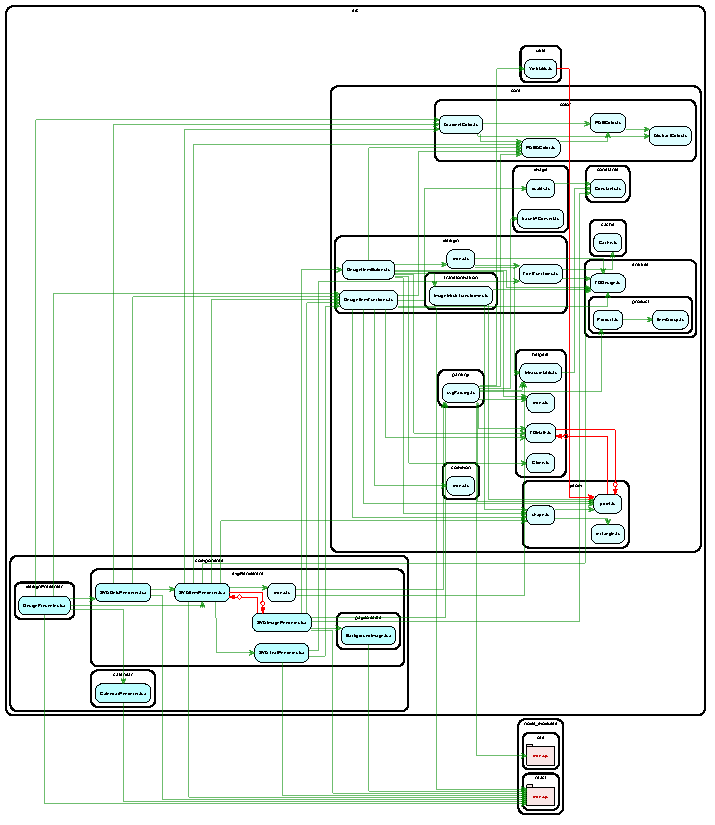
\includegraphics{diagrams/Ist-Architektur/design-presenter-analysis.pdf}
    \caption{Abhängigkeiten der Komponenten für Designdarstellung}
    \label{fig:Designdarstellung}
\end{figure}

Die React-Komponente \lstinline|DesignPresenter.tsx| erzeugt, basierend auf eine Designstruktur welche innerhalb der Datei \lstinline|src/core/entities/FDDesign.ts| definiert ist, die SVG-Struktur zur Darstellung im Browser. Die Datei \lstinline|FDDesign.ts| enthält eine Sammlung von Schnittstellen, welche die verschieden Elemente eine Designs beschreiben.   
Ein Darstellung der Strukturierung der Schnittstellen als Klassediagramm ist im Anhang unter \emph{D1\_FDDesign.pdf} enthalten.

Folgende Bausteine wurden aus den Abhängigkeiten der Designpräsentation extrahiert.
\begin{multicols}{2}
\begin{tabular}{ll}
\hline
\textbf{Bildverarbeitung} 
& core/image/* \\
\hline
\textbf{Cache} 
& core/cache/Cache.ts \\
\hline
\textbf{Designdarstellung} 
& components/svgRenderers/* \\
& components/designPresenter/* \\
\hline
\textbf{Designobjekt-Transformation}
& core/design/transformation/*	\\
\hline
\textbf{Designobjekterzeugung} 
& core/design/DesignItemBuilder.ts \\
\hline
\textbf{Designstruktur}
& core/entities/FDDesign.ts \\
\hline
\textbf{Farbstruktur}
& core/color/* \\
\hline
\textbf{JavaScript-Erweiterung} 
& core/helpers/Clone.ts \\
& core/helpers/index.ts \\
\hline
\textbf{Mathematik} 
& core/geom/*	               \\ 
& core/helpers/FDMath.ts	   \\ 
& utils/WebUtils.ts	           \\ 
\hline
\textbf{Maßeinheit-Konverter} 
& core/helpers/MeasureUtils.ts \\
\hline
\textbf{Produktstruktur} 
& core/entities/product/*	\\
\hline
\textbf{Schriftverarbeitung} 
& core/design/FontFunctions.ts \\
\hline
\textbf{SVG-Parser}
& core/parsing/svgParsing.ts \\
\hline
\textbf{XML-Parser}
& utils/WebUtils.ts \\
\end{tabular} 

%  \begin{tabular}{lr}
    % Pfad	                                            &   Komponente \\
    % \hline
    % core/image/*                                    &	Bildverarbeitung  \\
    % core/cache/Cache.ts	                            &   Cache  \\
    % components/svgRenderers/SVGTextRenderer.tsx	    &   Designdarstellung  \\
    % components/svgRenderers/SVGImageRenderer.tsx	&   Designdarstellung  \\
    % components/svgRenderers/SVGItemRenderer.tsx	    &   Designdarstellung  \\
    % components/svgRenderers/SVGDefsRenderer.tsx	    &   Designdarstellung  \\
    % components/svgRenderers/SVGPageRenderer.tsx	    &   Designdarstellung  \\
    % components/svgRenderers/index.ts        	    &   Designdarstellung  \\
    % components/designPresenter/DesignPresenter.tsx	&   Designdarstellung  \\
    % core/design/transformation/*	                &   Designobjekt-Transformation  \\
    % core/design/DesignItemBuilder.ts	            &   Designobjekterzeugung  \\
    % core/entities/FDDesign.ts	                    &   Designstruktur  \\
    % core/color/*	                                &   Farbstruktur  \\
    % core/helpers/Clone.ts	                        &   JavaScript-Erweiterung  \\
    % core/helpers/index.ts	                        &   JavaScript-Erweiterung  \\
    % core/geom/*	                                    &   Mathematik  \\
    % core/helpers/FDMath.ts	                        &   Mathematik  \\
    % utils/WebUtils.ts	                            &   Mathematik  \\
    % core/helpers/MeasureUtils.ts                    &	Maßeinheit-Konverter  \\
    % components/svgRenderers/pageAssets/*	        &   Produktdarstellung  \\
    % components/svgRenderers/SVGProductImageRenderer.tsx	    &   Produktdarstellung  \\
    % core/entities/product/*	                        &   Produktstruktur  \\
    % core/design/FontFunctions.ts	                &   Schriftverarbeitung  \\
    % core/parsing/svgParsing.ts	                    &   SVG-Parser  \\
    % utils/WebUtils.ts	                            &   XML-Parser  \\
%  \end{tabular} 
\end{multicols}